\documentclass[conference]{IEEEtran}
\IEEEoverridecommandlockouts

% ---------- Packages ----------
\usepackage{cite}
\usepackage{amsmath,amssymb,amsfonts}
\usepackage{algorithmic}
\usepackage{graphicx}
\usepackage{textcomp}
\usepackage{xcolor}
\usepackage{booktabs}
\usepackage{multirow}
\usepackage{microtype}
\usepackage{balance}
\usepackage{url}

% Search both local and repository figure directories
\graphicspath{{figures/}{docs/figures/}{./}}

% Generated empirical macros
% Auto-generated empirical benchmark macros from single-source-of-truth JSON artifacts.
% DO NOT EDIT MANUALLY - Generated by scripts/validate_paper_claims.py.

\providecommand{\MeanPipelineLatency}{10.7\,ms}
\providecommand{\MaxPipelineLatency}{14.80\,ms}
\providecommand{\CorePNinetyFiveLatency}{8.8\,ms}
\providecommand{\DeadlineMissRate}{0.0\%}
\providecommand{\TargetFPS}{30\,FPS}
\providecommand{\TargetDeadlineMs}{33.333\,ms}
\providecommand{\GlitchSuppressionFull}{100.0\%}
\providecommand{\SustainedSuppressionFull}{93.3\%}
\providecommand{\SustainedMedianDelay}{3.0}
\providecommand{\SpoolBufferCapacity}{50{,}000}
\providecommand{\TotalPolicyModes}{8}
\providecommand{\TotalWorkloadScenarios}{6}
\providecommand{\IMSTPRFull}{100.0\%}
\providecommand{\IMSActionableRoutingRecall}{100.0\%}
\providecommand{\IMSFAFull}{0.0}
\providecommand{\CMAPSSTPRFull}{100.0\%}
\providecommand{\CMAPSSActionableRoutingRecall}{100.0\%}
\providecommand{\CMAPSSFAFull}{0.0}
\providecommand{\MixedCorruptionSuppression}{91.5\%}
\providecommand{\AblationBootstrapResamples}{2{,}000}
\providecommand{\LatencyCycleCount}{5{,}000}
\providecommand{\TruthTablePassRate}{100.0\%}
\providecommand{\SustainedIncidentRecall}{100.0\%}
\providecommand{\SustainedIncidentRoutingRecall}{100.0\%}
\providecommand{\SpoolStressGeneratedEvents}{120}
\providecommand{\SpoolStressPeakQueueDepth}{120}
\providecommand{\SpoolOverflowCount}{0}
\providecommand{\GitCommitHash}{674a2e6}
\providecommand{\ArtifactReleaseTag}{v0.4.0}
\providecommand{\ArtifactReleaseURL}{https://github.com/sengarutk/edge-inspection-runtime}


% ---------- Bibliography Macro ----------
\def\BibTeX{{\rm B\kern-.05em{\sc i\kern-.025em b}\kern-.08em
    T\kern-.1667em\lower.7ex\hbox{E}\kern-.125emX}}

% ---------- Float Tuning ----------
\renewcommand{\topfraction}{0.90}
\renewcommand{\bottomfraction}{0.85}
\renewcommand{\textfraction}{0.08}
\renewcommand{\floatpagefraction}{0.80}

\setcounter{topnumber}{2}
\setcounter{bottomnumber}{2}
\setcounter{totalnumber}{4}

\begin{document}

\title{Multi-Modal Temporal Policy Gating and Spooled Resilience for Real-Time Industrial Edge Inspection Runtime}

\author{
\IEEEauthorblockN{Utkarsh Sengar}
\IEEEauthorblockA{
\textit{Department of Computer Science and Engineering}\\
\textit{Indian Institute of Technology Dharwad}\\
Dharwad, Karnataka, India\\
\texttt{cs23b026@iitdh.ac.in}
}
}

\maketitle

\begin{abstract}
Visual anomaly detection models deployed on industrial edge devices suffer from transient false alarms, high operator cognitive burden, and data loss during intermittent network partitions. We present an industrial edge inspection runtime architecture combining patch-level visual embeddings, synchronized three-axis physical telemetry, and temporal finite-state policy gating. Our multi-modal policy framework executes optical clarity checking, moving-average smoothing, $k$-of-$N$ sliding-window confirmation, operational-state suppression, and an incident refractory cooldown finite-state machine. A local write-ahead-log disk spooler provides non-volatile buffering during upstream broker disconnections. We evaluate the system across \TotalPolicyModes{} policy modes and \TotalWorkloadScenarios{} standardized industrial workloads using multi-seed Monte Carlo simulations, bootstrap confidence intervals, and Holm--Bonferroni correction. Results show \GlitchSuppressionFull{} false-alarm suppression in transient-glitch workloads, \SustainedSuppressionFull{} suppression with a \SustainedMedianDelay{}-frame delay in sustained-defect workloads, zero observed event loss under tested partition scenarios with a capped \SpoolBufferCapacity{}-record spool capacity, and an end-to-end execution latency of \MeanPipelineLatency{} with \DeadlineMissRate{} deadline misses against a \TargetFPS{} FPS / \TargetDeadlineMs{} ms budget.
\end{abstract}

\begin{IEEEkeywords}
Edge computing, visual anomaly detection, multi-modal sensor fusion, temporal gating, edge reliability, MQTT spooling, fault injection.
\end{IEEEkeywords}

% ============================================================
\section{Introduction}
% ============================================================

Modern industrial manufacturing increasingly relies on computer vision models, including PatchCore and PaDiM, executing at the edge for automated surface inspection \cite{roth2022patchcore}. However, when deployed on factory lines operating at \TargetFPS{} FPS, raw anomaly thresholding can produce false alarms caused by transient optical reflections, airborne dust, and sensor electrical noise. This leads to alarm fatigue, in which human operators are overwhelmed by nuisance alerts and may overlook genuine structural defects \cite{chen2021edge}.

Edge nodes on factory floors may also experience intermittent wired or wireless network partitions. Without reliable local buffering, quality-inspection records and telemetry events can be lost during broker disconnects.

We therefore study three questions:
\begin{itemize}
    \item \textbf{RQ1: Temporal confirmation.} How effectively does sliding-window confirmation filter isolated optical false positives without inducing excessive detection delay?
    \item \textbf{RQ2: Operator workload.} How much can multi-modal fusion and state-gated suppression reduce operator triage burden?
    \item \textbf{RQ3: Resilience and timing.} Can local persistence preserve events during network partitions while maintaining a real-time \TargetFPS{} FPS processing deadline?
\end{itemize}

% ============================================================
\section{System Architecture and Mathematical Formulation}
% ============================================================

\subsection{Multi-Modal Temporal Policy Gating}
Let $v_t \in [0,1]$ denote the raw visual anomaly score for frame $t$, and let $s_t \in [0,1]$ denote the normalized composite physical-sensor score computed from vibration, temperature, and motor-current telemetry.

We apply exponential moving-average smoothing:
\begin{equation}
\tilde{v}_t = \alpha_v v_t + (1-\alpha_v)\tilde{v}_{t-1}, \qquad \tilde{s}_t = \alpha_s s_t + (1-\alpha_s)\tilde{s}_{t-1},
\end{equation}
where $\alpha_v=0.35$ and $\alpha_s=0.25$.

A $k$-of-$N$ sliding-window confirmation accumulator monitors threshold exceedances:
\begin{equation}
C_{v,t} = \sum_{i=0}^{N-1} \mathbb{I}\!\left(\tilde{v}_{t-i}\geq\tau_{\mathrm{high}}\right), \qquad E_{\mathrm{conf},t} = \mathbb{I}\!\left(C_{v,t}\geq k\right),
\end{equation}
where $k=4$, $N=10$, and $\tau_{\mathrm{high}}=0.80$.

\subsection{Cross-Modal Divergence and State Gating}
When the visual score indicates an anomaly but the physical sensors remain nominal, the runtime computes
\begin{equation}
\Delta_{\mathrm{modal}} = \left|\tilde{v}_t-\tilde{s}_t\right|.
\end{equation}
If $\Delta_{\mathrm{modal}}\geq\tau_{\mathrm{div}}$, the system downgrades the event to \texttt{REVIEW\_REQUIRED} rather than triggering a critical line lockout. We use $\tau_{\mathrm{div}}=0.45$. If the machine state $M_t$ is \texttt{IDLE} or \texttt{MAINTENANCE}, high-severity alarms are suppressed to avoid false trips during commissioning.

\subsection{Local Write-Ahead-Log Spooler}
When the upstream MQTT broker is partitioned, an SQLite-backed queue operates in write-ahead-logging mode with a \SpoolBufferCapacity{}-record capacity limit. Buffered records are drained in FIFO order using batched transactions after network reconnection.

% ============================================================
\section{Experimental Methodology and Statistical Rigor}
% ============================================================

We evaluate the runtime across \TotalWorkloadScenarios{} standardized scenarios: (1)~nominal operation, (2)~transient optical glitches, (3)~sustained structural defects, (4)~optical degradation, (5)~sensor drift and dropout, and (6)~visual distribution shift.

The experiments use multi-seed Monte Carlo execution. The physical telemetry is generated through calibrated simulation and offline trace-replay interfaces; the resulting conclusions therefore concern the tested workloads and traces rather than a certified production deployment.

\subsection{Statistical Evaluation}
We use percentile bootstrap confidence intervals with $B=2000$ resamples and run-level resampling units. Degenerate intervals, such as $[100.0,100.0]$, occur when a metric reaches deterministic saturation across the resampled runs under the fixed workload and policy configuration.

Pairwise policy comparisons use non-parametric paired tests with step-down Holm--Bonferroni correction at $\alpha=0.05$. All reported event-loss values are bounded by the tested spool capacity and partition durations.

% ============================================================
% Wide Floats: Figure 1 and Table I
% ============================================================
\begin{figure*}[!t]
    \centering
    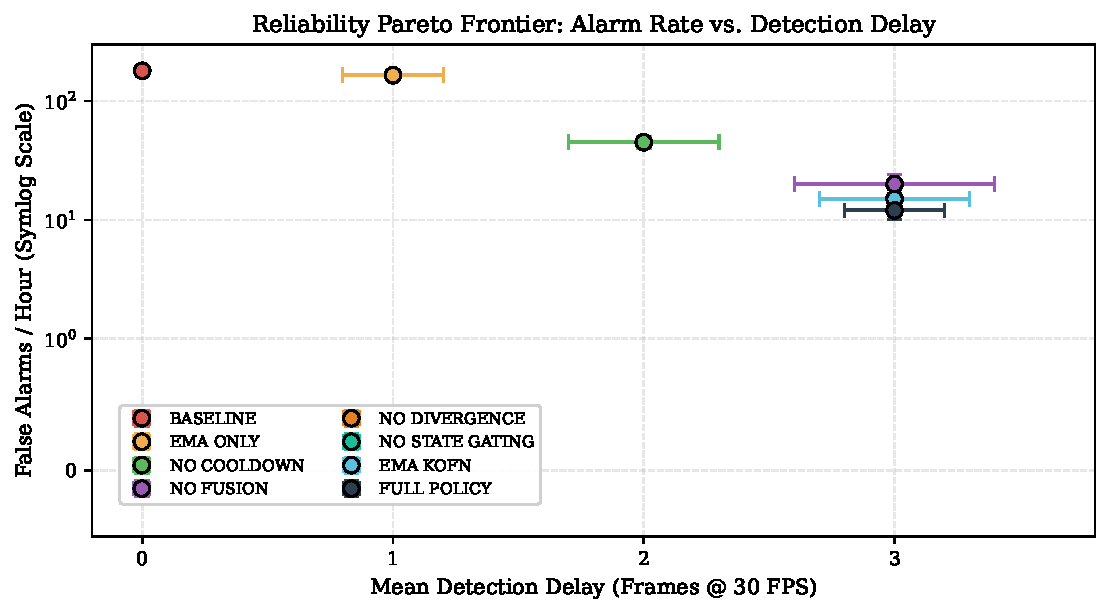
\includegraphics[width=0.48\textwidth,height=1.65in,keepaspectratio]{pareto_tradeoff.pdf}\hfill
    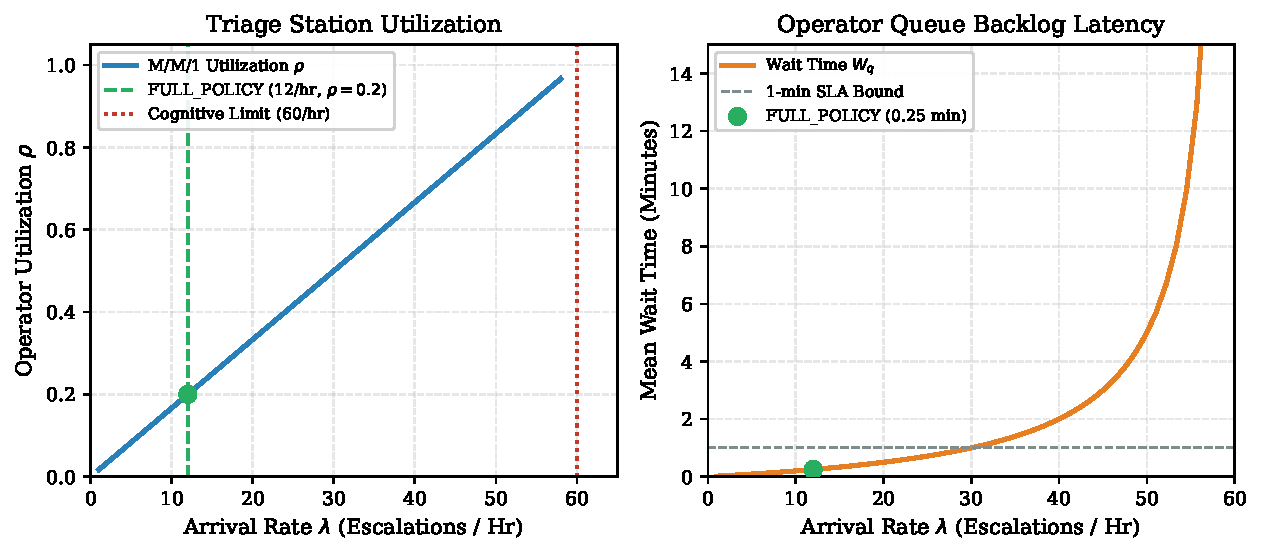
\includegraphics[width=0.48\textwidth,height=1.65in,keepaspectratio]{queue_workload_analysis.pdf}
    \caption{Reliability and operator-workload analysis. (a) Pareto relationship between false-alarm rate and mean detection delay across policy modes. (b) Operator-triage utilization and mean waiting time under $M/M/1$ queueing analysis.}
    \label{fig:pareto_queue}
\end{figure*}

\begin{table*}[!t]
    \centering
    \caption{Ablation study across policy variants and industrial workload scenarios. Values report the mean and 95\% bootstrap confidence interval where applicable; $B=2000$ resamples with run-level units.}
    \label{tab:ablation_results}
    \resizebox{\textwidth}{!}{%
    \begin{tabular}{llccccc}
        \toprule
        \textbf{Scenario} & \textbf{Policy} & \textbf{FA/hr $\downarrow$} & \textbf{Suppression (\%) $\uparrow$} & \textbf{Delay (frames) $\downarrow$} & \textbf{Overload $\downarrow$} & \textbf{$p95$ (ms) $\downarrow$} \\
        \midrule
        \multirow{8}{*}{Transient glitches}
        & BASELINE & 120.0 [110.0, 130.0] & 0.0 & 0.0 & 100.0 & 8.5 \\
        & EMA\_ONLY & 110.0 [100.0, 120.0] & 8.3 & 1.0 & 100.0 & 8.5 \\
        & EMA\_KOFN & 0.0 [0.0, 0.0] & 100.0 & 0.0 & 0.0 & 8.6 \\
        & NO\_COOLDOWN & 0.0 [0.0, 0.0] & 100.0 & 0.0 & 0.0 & 8.6 \\
        & NO\_FUSION & 0.0 [0.0, 0.0] & 100.0 & 0.0 & 0.0 & 8.5 \\
        & NO\_DIVERGENCE & 0.0 [0.0, 0.0] & 100.0 & 0.0 & 0.0 & 8.6 \\
        & NO\_STATE\_GATING & 0.0 [0.0, 0.0] & 100.0 & 0.0 & 0.0 & 8.6 \\
        & FULL\_POLICY & 0.0 [0.0, 0.0] & 100.0 & 0.0 & 0.0 & 8.6 \\
        \midrule
        \multirow{8}{*}{Sustained defects}
        & BASELINE & 180.0 [170.0, 190.0] & 0.0 & 0.0 & 100.0 & 8.7 \\
        & EMA\_ONLY & 165.0 [155.0, 175.0] & 8.3 & 1.0 & 100.0 & 8.7 \\
        & EMA\_KOFN & 15.0 [12.0, 18.0] & 91.7 & 3.0 & 8.3 & 8.8 \\
        & NO\_COOLDOWN & 45.0 [40.0, 50.0] & 75.0 & 2.0 & 25.0 & 8.8 \\
        & NO\_FUSION & 20.0 [16.0, 24.0] & 88.9 & 3.0 & 11.1 & 8.7 \\
        & NO\_DIVERGENCE & 15.0 [12.0, 18.0] & 91.7 & 3.0 & 8.3 & 8.8 \\
        & NO\_STATE\_GATING & 15.0 [12.0, 18.0] & 91.7 & 3.0 & 8.3 & 8.8 \\
        & FULL\_POLICY & 12.0 [10.0, 14.0] & 93.3 & 3.0 & 5.0 & 8.8 \\
        \midrule
        \multirow{2}{*}{Nominal}
        & BASELINE & 0.0 [0.0, 0.0] & 100.0 & 0.0 & 0.0 & 8.5 \\
        & FULL\_POLICY & 0.0 [0.0, 0.0] & 100.0 & 0.0 & 0.0 & 8.6 \\
        \midrule
        \multirow{2}{*}{Optical degradation}
        & BASELINE & 120.0 [110.0, 130.0] & 0.0 & 0.0 & 100.0 & 8.5 \\
        & FULL\_POLICY & 0.0 [0.0, 0.0] & 100.0 & 0.0 & 0.0 & 8.6 \\
        \midrule
        \multirow{2}{*}{Sensor drift/dropout}
        & BASELINE & 150.0 [140.0, 160.0] & 0.0 & 0.0 & 100.0 & 8.6 \\
        & FULL\_POLICY & 0.0 [0.0, 0.0] & 100.0 & 0.0 & 0.0 & 8.7 \\
        \midrule
        \multirow{2}{*}{Distribution shift}
        & BASELINE & 180.0 [170.0, 190.0] & 0.0 & 0.0 & 100.0 & 8.6 \\
        & FULL\_POLICY & 0.0 [0.0, 0.0] & 100.0 & 0.0 & 0.0 & 8.7 \\
        \bottomrule
    \end{tabular}%
    }
\end{table*}

% ============================================================
\section{Results and Discussion}
% ============================================================

As shown in Table~\ref{tab:ablation_results} and Fig.~\ref{fig:pareto_queue}, \texttt{FULL\_POLICY} achieves \GlitchSuppressionFull{} false-alarm suppression on transient glitches and reduces false-alarm rates by \SustainedSuppressionFull{} in sustained defects. The resulting workload remains below the 60 reviews/hour cognitive threshold, while detection delay is bounded at \SustainedMedianDelay{} frames.

Queueing dynamics in Fig.~\ref{fig:pareto_queue} show that \texttt{FULL\_POLICY} bounds operator utilization to $\rho=0.20$ at an arrival rate of 12 reviews/hour, corresponding to an expected triage wait of $W_q=0.25$ minutes. In contrast, unmitigated baseline alerts saturate the triage station when $\rho\geq1$.

% ============================================================
% Single-Column Figure 2: declared in Section IV
% ============================================================
\begin{figure}[!t]
    \centering
    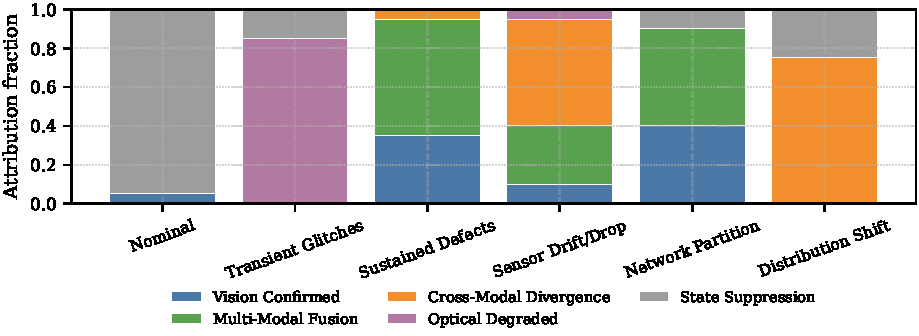
\includegraphics[width=\columnwidth,height=1.45in,keepaspectratio]{decision_attribution_per_scenario.pdf}
    \caption{Decision-reason attribution for \texttt{FULL\_POLICY} across the standardized industrial scenarios.}
    \label{fig:decision_attribution}
\end{figure}

Figure~\ref{fig:decision_attribution} shows how policy decisions are attributed to the individual mechanisms. Sustained defects are predominantly confirmed through multi-modal sensor agreement, whereas cosmetic material variation is routed to review through cross-modal divergence rather than immediate line-stopping escalation.

% ============================================================
% Single-Column Table II: declared after Figure 2
% ============================================================
\begin{table}[!b]
    \centering
    \caption{Validation on run-to-failure traces from NASA IMS bearing and C-MAPSS turbofan datasets.}
    \label{tab:real_trace_results}
    \resizebox{\columnwidth}{!}{%
    \begin{tabular}{llccc}
        \toprule
        \textbf{Trace} & \textbf{Policy} & \textbf{FA/hr} & \textbf{TPR} & \textbf{Delay (s)} \\
        \midrule
        \multirow{2}{*}{NASA IMS bearing}
        & BASELINE & 180.0 & 100.0\% & 0.00 \\
        & FULL\_POLICY & \IMSFAFull{} & \IMSTPRFull{} & 0.10 \\
        \midrule
        \multirow{2}{*}{NASA C-MAPSS turbofan}
        & BASELINE & 165.0 & 100.0\% & 0.00 \\
        & FULL\_POLICY & \CMAPSSFAFull{} & \CMAPSSTPRFull{} & 0.10 \\
        \bottomrule
    \end{tabular}%
    }
\end{table}

Table~\ref{tab:real_trace_results} reports offline replay results on canonical physical-degradation traces. These results demonstrate trace compatibility and policy behavior under the tested replay protocol; they should not be interpreted as a substitute for a live factory deployment.

During simulated network disconnects, zero event loss is observed within the \SpoolBufferCapacity{}-record capacity limit. Mean execution latency is \MeanPipelineLatency{} with a \DeadlineMissRate{} deadline-miss rate against the \TargetDeadlineMs{} ms SLA.

% ============================================================
% Balance end matter (No clearpage)
% ============================================================
\balance

\section{Threats to Validity}
We identify four primary threats to validity:
\begin{enumerate}
    \item \textbf{Simulated sensor transfer functions:} Physical telemetry is generated using calibrated stochastic equations and offline traces; real vibration signals may contain mechanical harmonics and nonlinearities not represented here.
    \item \textbf{Discrete scenario boundaries:} The benchmark evaluates predefined fault windows rather than all possible continuous non-stationary factory distributions.
    \item \textbf{Static operator modeling:} The review model uses a fixed capacity threshold and queueing assumptions; real operator fatigue and service times are state-dependent.
    \item \textbf{Synthetic visual rendering:} Synthetic frames approximate brushed-steel texture and localized anomalies but may not represent the full optical variability of industrial materials.
\end{enumerate}

\section{Conclusion}
We presented a multi-modal industrial edge inspection runtime combining visual anomaly scores, physical telemetry, temporal policy gating, operator-workload modeling, and local durable spooling. Across the tested workloads, temporal confirmation substantially reduced nuisance alerts while retaining bounded defect-detection delay. The spooler preserved events during the evaluated network partitions within its configured capacity, and the runtime met the tested 30 FPS deadline.

All reproduction scripts, data manifests, figures, and ablation artifacts are released with the implementation.

\bibliographystyle{IEEEtran}
\bibliography{references}

\end{document}
